\chapter{Calculations for dynamics}\label{app:dynamics_calc}
This appendix will contain calculations for the chapter concerning dynamics of the system.

\section{Inertia of the pan/tilt}
A sketch of the pan/tilt system is shown in the figure below.
\begin{figure}[htb]
	\centering
	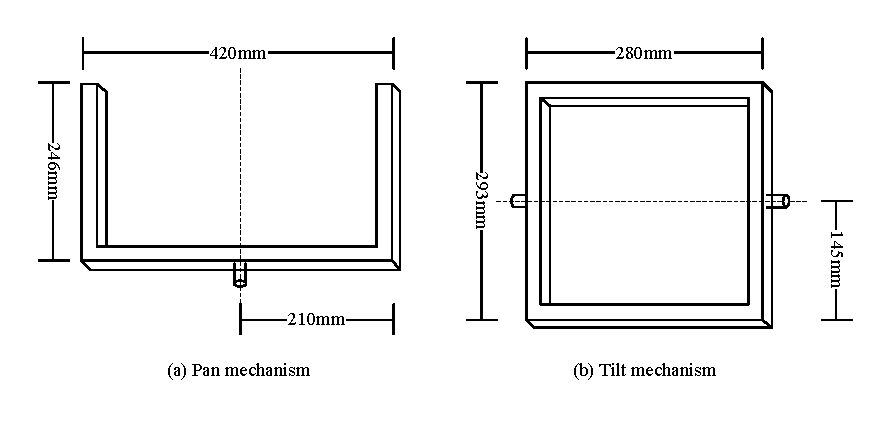
\includegraphics[width=\textwidth]{graphics/pan_tilt_sketch.pdf} %trim=l b r t (can cut off from every side)
	\caption{Simple sketch of the pan/tilt system with measurements. The dimension of the profile is 40 x 40 mm. The profile that is used weigh $1.565\sfrac{kg}{m}$}
	\label{fig:pan_tilt_sketch}			% figure labels are of the form \label{fig:*}
\end{figure}

\subsection{Pan inertia}
To calculate the inertia of the pan mechanism some considerations have to be made about how to model it. Figure \ref{fig:pan_tilt_sketch}(a) will be modelled in a way so the bar connected to the turning shaft will be considered as a rod with two point masses connected to each end of the bar, the total inertia of the pan mechanism will be calculated from the parallel axis theorem. The parallel axis theorem says:
\begin{equation}
	J = J_{COM} + M d^{2} \label{eq:parallel_axis_theorem}
\end{equation}
where $J$ is the total inertia, $J_{COM}$ is the inertia of the base bar, $M$ is the mass that is displaced and $d$ is the displacement. $J_{COM}$ is calculated as follows:
\begin{equation}
	J_{COM} = \dfrac{M L^{2}}{12} \Longrightarrow J_{COM} = \dfrac{(1.565\sfrac{kg}{m} \cdot 0.42m) \cdot (0.42m)^{2}}{12} = 0.058 kg \cdot m^{2}
\end{equation}
Calculation of the total inertia is calculated as follows:
\begin{align}
J_{Pan} &= J_{COM} + 2 \cdot M d^{2} \Longrightarrow \\
J_{Pan} &= 0.058 kg \cdot m^{2} + 2 \cdot (1.565\sfrac{kg}{m} \cdot 0.246m) \cdot (0.21m)^{2} \Longrightarrow \label{eq:pan_inertia_temp} \\ 
J_{Pan} &= 0.092 kg \cdot m^{2}\label{eq:pan_inertia}
\end{align}
\ref{eq:pan_inertia_temp} has its second term multiplied with two, this is done as the pan mechanism has two masses that is displaced equally from the axis of rotation.

\subsection{Tilt inertia}
The inertia of the tilt part of the system is considered as a rod with two point masses displaced equally from the axis of rotation. The inertia is calculated the following way:
\begin{equation}
	J_{COM} = \dfrac{ML^{2}}{12} = \dfrac{2 \cdot 1.565 \sfrac{kg}{m} \cdot 0.293 m \ (0.293m)^{2}}{12} = 0.079 kg \cdot m^{2}
\end{equation}
Adding the displaced masses to the inertia is done with the parallel axis theorem as follows:
\begin{align}
J_{Tilt} &= J_{COM} + 2 \cdot M d^{2} \Longrightarrow \\
J_{Tilt} &= 0.079 kg \cdot m^{2} + 2 \cdot (1.565\sfrac{kg}{m} \cdot 0.280m) \cdot (0.145m)^{2} \Longrightarrow \label{eq:tilt_inertia_temp} \\ 
J_{Tilt} &= 0.097 kg \cdot m^{2}\label{eq:tilt_inertia}
\end{align}

\section{Gears}
The load at the motors are the reflected inertia through the gears plus the inertia of the rotor in the motor, the rotors inertia is omitted. The two gears are connected together and then connected between the motor and the inertia. The gearing system is equal on the pan and the tilt. Figure \ref{fig:app_gears} show a simplification of the gearing.
\begin{figure}[htb]
	\centering
	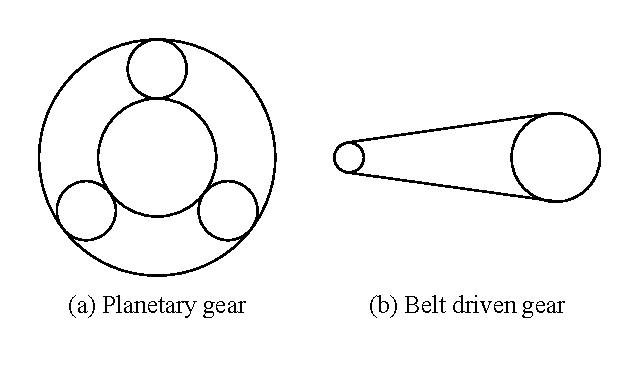
\includegraphics[scale=1,trim=0 0 0 0]{graphics/gears.pdf} %trim=l b r t (can cut off from every side)
	\caption{Simplification of the gears in the pan/tilt system. (a) Show a simplification of a planetary gear which has, according to the datasheet of the motor which is included on the CD, a gearing of $N = 30:1$. (b) The gearing of the belt driven gear is experimental measured and calculated to be $N = 1:3$}
	\label{fig:app_gears}			% figure labels are of the form \label{fig:*}
\end{figure}
The load reflected through a gear is given by\footnote{REF NEEDED!!!   (http://www.techno-isel.com/tic/h834/PDF/H834P009.pdf)}:
\begin{equation}
	J_R = \frac{J_L}{N^{2}}
\end{equation}
where $J_R$ is the reflected load behind the gear, $J_L$ is the load in front of the gear, N is the gear ratio. As the pan and tilt gearing is equal the following expression is derived the total gearing between the motor and the mass:
\begin{equation}
	J_R = \frac{\frac{J_L}{(\sfrac{1}{3})^{2}}}{30^{2}} = \frac{J_L}{(\sfrac{1}{3})^{2} \cdot 30^{2}}\label{app:eq_reflected_inertia_temp}
\end{equation}

\subsection{Reflected inertia (pan)}
If the inertial load from the pan is substituted into equation \ref{app:eq_reflected_inertia_temp} the following is obtained:
\begin{equation}
	J_{Pan} = \frac{0.092 kg \cdot m^{2}}{(\sfrac{1}{3})^{2} \cdot 30^{2}} = 0.920 \cdot 10^{-3} kg \cdot m^{2} \label{app:eq_reflected_pan_inertia}
\end{equation}

\subsection{Reflected inertia (tilt)}
If the inertial load from the tilt is substituted into equation \ref{app:eq_reflected_inertia_temp} the following is obtained:
\begin{equation}
	J_{Tilt} = \frac{0.097 kg \cdot m^{2}}{(\sfrac{1}{3})^{2} \cdot 30^{2}} = 0.970 \cdot 10^{-3} kg \cdot m^{2} \label{app:eq_reflected_tilt_inertia}
\end{equation} 

\section{Constants for model}
